\documentclass[conference]{IEEEtran}
\usepackage{cite}
\usepackage{amsmath,amssymb}
\usepackage{booktabs}
\usepackage{graphicx}
\usepackage{tikz}
\usetikzlibrary{arrows.meta,positioning,shapes.geometric}
\usepackage{url}
\usepackage{xcolor}
\usepackage{listings}
\usepackage{balance}

\title{IntentFlow: Deterministic Constrained Planning and Evidence-Aware Execution in a Fixed SDN Testbed}
\author{
\IEEEauthorblockN{Izhaar Ahmed Shaik}
\IEEEauthorblockA{Department of Data Science and Artificial Intelligence\\
Indian Institute of Information Technology Dharwad (IIIT Dharwad)\\
izhaarahmedshaik@gmail.com}
\and
\IEEEauthorblockN{Sasi Rekha Sadanala}
\IEEEauthorblockA{Department of Data Science and Artificial Intelligence\\
Indian Institute of Information Technology Dharwad (IIIT Dharwad)\\
sasirekhasadanala10@gmail.com}
\and
\IEEEauthorblockN{Manasa Saragalla}
\IEEEauthorblockA{Department of Data Science and Artificial Intelligence\\
Indian Institute of Information Technology Dharwad (IIIT Dharwad)\\
23bds051@iiitdwd.ac.in}
\and
\IEEEauthorblockN{Sudharshana Suryanarayanan}
\IEEEauthorblockA{Department of Data Science and Artificial Intelligence\\
Indian Institute of Information Technology Dharwad (IIIT Dharwad)\\
23bds059@iiitdwd.ac.in}
}

\lstset{
basicstyle=\ttfamily\footnotesize,
breaklines=true,
columns=fullflexible
}

\begin{document}
\maketitle

\begin{abstract}
IntentFlow is a typed intent-to-path and Software-Defined Networking (SDN)
prototype that separates natural-language interpretation, deterministic
planning, physical-path compilation, deployment, active measurement, and
execution evidence. It provides a DESIGN-mode configured-metric planner and a
generalized live execution workflow over a fixed Mininet/Open vSwitch/Ryu
diamond topology. A third, legacy command-line workflow implements a bandwidth
feedback experiment that adjusts the QoS cap of a known competing flow.
These workflows are related implementation components, but they are not one
integrated controller. The deterministic core validates canonical intents,
enumerates exact physical paths, evaluates conjunctive hard constraints,
and ranks eligible candidates by an optional metric objective. Missing
metric facts fail closed. Live candidate and final measurements use ping or
iperf3, while OpenFlow rules are checked with switch-flow readback.
The legacy CLI bandwidth sweep retained 27 completed runs and 14
infrastructure timeouts. Across the four systematic scenarios, every
per-scenario satisfaction-rate comparison showed zero improvement for
CLOSED\_LOOP operation. This sweep is separate from the generalized LIVE
demonstrations: eight retained generalized execution records contain seven
SUCCEEDED and one FAILED result, and are individual demonstrations rather
than repeated trials. Individual manual demonstrations showed both a
one-iteration correction success and a three-iteration bounded failure.
Accordingly, this paper makes only narrow implementation and evidence claims:
it does not claim general closed-loop benefit, statistical significance,
scalability, or superiority over independently implemented routing baselines.
\end{abstract}

\begin{IEEEkeywords}
intent-based networking, software-defined networking, constrained routing,
path selection, OpenFlow, Mininet, network measurement
\end{IEEEkeywords}

\section{Introduction}
Intent-based networking asks operators to express network outcomes rather
than switch-level instructions. SDN provides centralized control, but natural
language can be ambiguous and should not directly authorize configuration
commands. IntentFlow addresses this separation as a systems engineering
problem: translate supported requests into a versioned typed intent, plan over
a topology, compile an exact physical route, deploy and verify it, measure the
network, and retain evidence. The implementation also preserves the distinction
between a configured topology fact and a result observed from a live network.

The repository implements three distinguishable workflows:
\begin{enumerate}
\item \emph{DESIGN mode}, in which versioned topology graphs support
side-effect-free previews using configured bandwidth, delay, and loss values;
\item \emph{generalized LIVE execution}, in which the privileged worker builds
the fixed diamond testbed, measures candidate routes, performs exact flow
readback, and deploys a selected route; and
\item a \emph{legacy CLI bandwidth/latency workflow}, with
ONE\_SHOT and CLOSED\_LOOP modes and a QoS-based competing-flow correction
mechanism.
\end{enumerate}
The API and generalized worker do not invoke this legacy correction mode.
Calling the legacy bandwidth loop ``generalized closed-loop intent execution''
would therefore be incorrect.

\subsection{Research Objectives}
This study asks:
\begin{itemize}
\item RQ1: Can a typed intent model, exact path enumeration, and deterministic
constraint evaluation produce a bounded, fail-closed planning result?
\item RQ2: Can a live SDN executor separate static feasibility, candidate
measurement, exact flow readback, final connectivity, and cleanup evidence?
\item RQ3: In the fixed live diamond testbed, do ONE\_SHOT and
CLOSED\_LOOP bandwidth measurements differ in retained intent satisfaction?
\end{itemize}

The precise contributions are (i) a canonical intent and capability boundary
between interpretation and configuration, (ii) exact physical-path
enumeration with deterministic ranking and bounded search, (iii) a live
probe/deploy/readback/evidence lifecycle, and (iv) an honest empirical
comparison of two legacy bandwidth policies. These are implementation and
methodological contributions, not demonstrated algorithmic superiority.

\section{Related Work}
Intent-based networking aims to express desired outcomes instead of device
configuration. The IETF terminology and architecture framework by Clemm,
Ciavaglia, Granville, and Tantsura distinguishes intent concepts from
traditional policy abstractions and motivates lifecycle and outcome
validation \cite{rfc9315}. IntentFlow uses a narrower, versioned Pydantic
model whose capabilities and metric semantics are resolved deterministically.

OpenFlow provides a controller-switch flow-management abstraction for
programming forwarding behavior \cite{mckeown2008openflow}. IntentFlow uses
Ryu's ofctl REST interface to install OpenFlow 1.3 IPv4 and ARP rules and
verifies exact flow-table readback. Flow readback is evidence of the installed
rules on the queried switches; it is not formal network-wide verification.
Static approaches such as Header Space Analysis reason about reachability
and invariants from forwarding rules \cite{kazemian2012hsa}. IntentFlow does
not implement such a global verifier.

Constraint-aware routing has long used multi-constraint shortest-path
formulations. Kuipers and Van Mieghem identify the intractability of exact
multi-constrained routing and the role of efficient approximation
\cite{kuipers2002mamcra}. Yen's $K$-shortest loopless paths algorithm provides
the classical bounded path-enumeration concept \cite{yen1971}; IntentFlow
instead enumerates all loop-free exact paths up to a configurable limit and
returns incomplete search rather than pretending that the bounded result is
globally complete.

Network resource provisioning and QoS routing require separating static
resource feasibility from measured runtime behavior. IntentFlow's live
workflow explicitly performs candidate measurement and final remeasurement;
configured capacity is not substituted for throughput evidence. For live
monitoring, passive flow counters can complement active probes. OpenSketch
separates measurement primitives from applications \cite{yu2013opensketch},
whereas IntentFlow primarily uses ping and iperf3 active probes and the Ryu
flow-table query. This is a complementary, narrower mechanism.

SDN architecture surveys separate a programmable control plane from data-plane
forwarding and document the shift from vendor-specific configuration to
centralized policies \cite{kreutz2015,nunes2014,feamster2014}. IntentFlow
operates within this architecture but implements only one fixed testbed and
does not claim a general SDN control platform. Commercial and research
controllers similarly expose policy APIs, but IntentFlow adds a typed
intent/capability stage and explicit candidate evidence.

Policy-based early systems such as Ethane and Frenetic established centralized
flow policy and language/compiler abstractions
\cite{casado2007ethane,foster2011frenetic}. Frenetic and subsequent declarative
systems compile network policies; IntentFlow additionally separates
intent interpretation from exact physical routing and retains deployment and
measurement evidence. Google's B4 and Hedera show that centralized traffic
engineering can be deployed at scale \cite{jain2013b4,hedera2010}; IntentFlow
does not provide or evaluate comparable traffic engineering at WAN scale.
Likewise, ElasticTree addresses data-center power-aware routing
\cite{heller2010elastictree}, whereas IntentFlow is narrowly focused on
bandwidth, latency, loss, and exact candidate selection.

Control-plane verification systems provide stronger properties than IntentFlow.
VeriFlow validates invariants incrementally as rules change
\cite{khurshid2013veriflow}, NetPlumber models rule updates continuously
\cite{netplumber2013}, Anteater checks network states from forwarding
snapshots \cite{mai2011anteater}, and Batfish performs offline
configuration and data-plane analysis \cite{batfish2015}. ATPG demonstrates
test-packet generation for fault coverage \cite{zeng2012atpg}.
IntentFlow's flow readback and ping/iperf3 probes verify only its own host-pair
deployment and connectivity; they do not replace these network-wide methods.
NetKAT provides a formal data-plane language and equational theory
\cite{anderson2014netkat}; this work has no comparable formal semantics or
proof system.

QoS and multi-constraint routing often depend on approximations or performance
algebra. Wang and Crowcroft formalized QoS path selection
\cite{wang1996qos}, and Sobrinho developed algebraic routing conditions
\cite{sobrinho2001}. Kuipers and Van Mieghem's MAMCRA, discussed above,
addresses multi-constrained multicast routing. These works differ from
IntentFlow's small exact enumerator: its main verification is candidate
identity, configured/static feasibility, live measurement, and bounded search.

Closed-loop network control has also been studied outside the bandwidth
feedback mechanism. Kinetic expresses dynamic network policies as
finite-state-machine policies checked in operation \cite{kim2015kinetic}.
IntentFlow instead uses a deterministic QoS correction loop that lowers a
known competing flow; the retained experiment does not demonstrate general
feedback-controller convergence or fairness.

Finally, LLM-assisted network configuration must constrain model authority.
NetConfEval benchmarks LLMs on network configuration tasks and shows that
configuration correctness requires evaluation beyond text generation
\cite{wang2024netconfeval}. IntentFlow confines external and mock providers
to parsing and schema validation. External providers are optional; the mock
provider is deterministic regex/rule parsing and is not an LLM experiment.

\section{System Architecture}
\subsection{Three Execution Modes}
Fig.~\ref{fig:architecture} summarizes the code execution order. In
DESIGN mode, an active catalog topology is passed directly to
\texttt{plan\_on\_topology()}; no privileged worker, Ryu, or switch operation
is involved. In generalized LIVE mode, the API asks an allowlisted Unix-socket
worker to build the fixed diamond topology and execute
\texttt{run\_generalized\_constraint\_demo()}. In the legacy CLI workflow,
\texttt{backend.cli} invokes objective-specific bandwidth or latency code
and, for CLOSED\_LOOP, the known-competing-flow correction loop.

\begin{figure}[t]
\centering
\resizebox{\columnwidth}{!}{
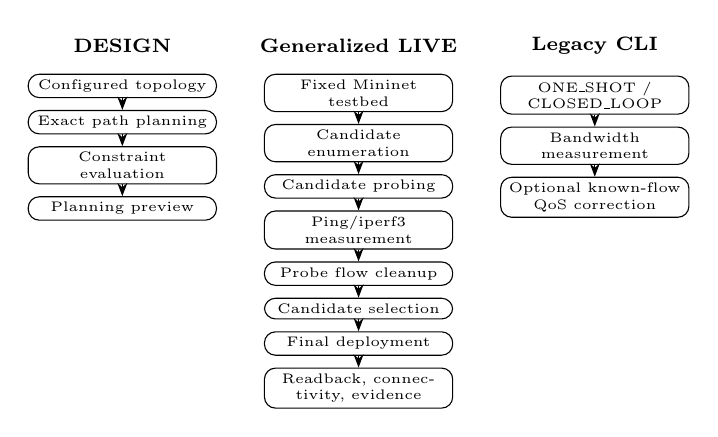
\begin{tikzpicture}[node distance=1.5mm, every node/.style={font=\tiny},
branch/.style={draw, rounded corners, align=center, inner sep=2pt, text width=2.25cm}]
\node[font=\scriptsize\bfseries] (dh) at (-3.0,0) {DESIGN};
\node[branch, below=of dh] (dtop) {Configured topology};
\node[branch, below=of dtop] (dpath) {Exact path planning};
\node[branch, below=of dpath] (dc) {Constraint evaluation};
\node[branch, below=of dc] (dp) {Planning preview};
\draw[-{Stealth}] (dtop)--(dpath); \draw[-{Stealth}] (dpath)--(dc); \draw[-{Stealth}] (dc)--(dp);

\node[font=\scriptsize\bfseries] (lh) at (0,0) {Generalized LIVE};
\node[branch, below=of lh] (ltop) {Fixed Mininet testbed};
\node[branch, below=of ltop] (lenum) {Candidate enumeration};
\node[branch, below=of lenum] (lprobe) {Candidate probing};
\node[branch, below=of lprobe] (lmeasure) {Ping/iperf3 measurement};
\node[branch, below=of lmeasure] (lclean) {Probe flow cleanup};
\node[branch, below=of lclean] (lselect) {Candidate selection};
\node[branch, below=of lselect] (lfinal) {Final deployment};
\node[branch, below=of lfinal] (lverify) {Readback, connectivity, evidence};
\draw[-{Stealth}] (ltop)--(lenum); \draw[-{Stealth}] (lenum)--(lprobe);
\draw[-{Stealth}] (lprobe)--(lmeasure); \draw[-{Stealth}] (lmeasure)--(lclean);
\draw[-{Stealth}] (lclean)--(lselect); \draw[-{Stealth}] (lselect)--(lfinal);
\draw[-{Stealth}] (lfinal)--(lverify);

\node[font=\scriptsize\bfseries] (ch) at (3.0,0) {Legacy CLI};
\node[branch, below=of ch] (cmode) {ONE\_SHOT / CLOSED\_LOOP};
\node[branch, below=of cmode] (cbw) {Bandwidth measurement};
\node[branch, below=of cbw] (cqos) {Optional known-flow QoS correction};
\draw[-{Stealth}] (cmode)--(cbw); \draw[-{Stealth}] (cbw)--(cqos);
\end{tikzpicture}
}
\caption{Separate implementation branches. DESIGN has no live deployment.
Generalized LIVE installs exact probe/final rules and verifies evidence.
The legacy CLI branch alone implements ONE\_SHOT and bounded competing-flow
QoS correction.}
\label{fig:architecture}
\end{figure}

\subsection{Intent and Capability Boundary}
\texttt{CanonicalIntent} contains a schema version, source/destination scope,
traffic selector, ordered metric constraints, at most one optimization
objective, requested actions, and legacy metadata. Provider output is parsed
as \texttt{StructuredIntent} and normalized after validation. Requested actions
are represented but are not executable handlers. The capability resolver
distinguishes recognition, static planning, live measurement, and execution.
Capability-ready means that declared checks passed, not that deployment
succeeded.

\subsection{Topology and Exact Physical Paths}
The topology model stores switch DPIDs and ports, host attachments, switch
links, and optional endpoint and link metrics. An exact enumerated route
contains source host and attachment, loop-free switch sequence, destination
attachment and host, while preserving switch-port and link identity.
Parallel links remain distinguishable. The enumerator rejects invalid
topologies, administrative-down links or attachments, and ambiguous port
ownership.

The live diamond has five switches and four hosts. Paths
$A=h1-s1-s2-s4-h4$ and $B=h1-s1-s3-s5-s4-h4$ have TCLink configured
bottlenecks of 10 and 50 Mbps, respectively. A background $h2-h3$ flow
shares links with Path A. These 10/50 Mbps values are configuration, not
iperf3 measurements.

\section{Mathematical Formulation}
\subsection{Configured DESIGN Metrics}
For a complete physical path $p$, let $E(p)$ be switch links and $a_s,a_d$
be endpoint attachments. When every required value is known and valid,
DESIGN bandwidth is
\begin{equation}
B_{\mathrm{cfg}}(p)=\min\left(
\{B_e:e\in E(p)\}\cup\{B_{a_s},B_{a_d}\}\right).
\end{equation}
Configured delay is
\begin{equation}
D_{\mathrm{cfg}}(p)=\sum_{e\in E(p)}D_e+D_{a_s}+D_{a_d},
\end{equation}
and configured loss is
\begin{equation}
L_{\mathrm{cfg}}(p)=100\left(1-\prod_{e\in E(p)\cup\{a_s,a_d\}}
(1-L_e/100)\right).
\end{equation}
This expression assumes that per-link and endpoint loss events are
independent for the probability-survival product. It is a multiplicative
configured-loss model, not an empirical measurement of correlated loss or
of temporal burst behavior.
Missing or invalid required values return UNKNOWN. This fail-closed
correction prevents incomplete attachment data from becoming an apparently
satisfied constraint.

\subsection{Constraint and Objective Evaluation}
For observation $x$, constraint comparison $c$, and threshold $v$, the scalar
operators are $x>v$, $x\ge v$, $x<v$, $x\le v$, and
$|x-v|\le\epsilon$ for equality. BETWEEN is inclusive. A candidate is eligible
only if every hard constraint is SATISFIED. UNKNOWN, stale, invalid, or
ambiguous observations do not establish eligibility.

An objective orders eligible candidates by ascending configured or measured
value for MINIMIZE and descending value for MAXIMIZE. Equal values are ordered
by ascending SHA-256 physical-path fingerprint. A fingerprint is a stable
tie-break, not a domain-specific preference. If no objective is supplied,
enumeration order determines the selected candidate.

\subsection{Live Candidate Selection and Enumeration}
The generalized executor first performs static feasibility where sufficient
facts exist. It may skip a candidate that cannot satisfy a known bandwidth
lower bound. Other candidates are probed sequentially. Enumeration is bounded
at 64 candidates by default; if truncation occurs, the result is
INCOMPLETE\_SEARCH and no selected path is reported. This is an implemented
bound, not a global-optimality guarantee.

\section{Methodology}
\subsection{DESIGN Planning}
The frontend/API can activate a versioned topology and submit a preview.
\texttt{plan\_on\_topology()} enumerates exact paths, aggregates available
configured facts, evaluates constraints, ranks eligible candidates, and
returns a deterministic planning result. Activation has no Mininet or flow
side effects.

\subsection{Generalized LIVE Execution}
The generalized orchestration:
\begin{enumerate}
\item validates the candidate request and fresh topology snapshot;
\item enumerates and statically assesses candidates;
\item preflights a probe and compiles bidirectional IPv4/ARP rules;
\item deploys rules with a probe cookie and performs switch-table readback;
\item performs a real ping or iperf3 measurement;
\item cleans the probe with cookie and DPID scoping; and
\item redoes preflight, deploys the selected route, verifies final
connectivity, and persists JSON/Markdown evidence.
\end{enumerate}
Candidate measurements are shared only by metric and identity checks; they
are not assumed to remain valid when snapshot or request identity changes.
For packet-loss constraints, the generalized workflow runs the ping used for
latency with a default of 10 transmitted packets and parses the packet-count
summary. A packet-loss observation is retained only when the summary reports
the requested packet count, received counts within the transmitted range,
and loss within $0.5$ percentage points of
$100(\text{sent}-\text{received})/\text{sent}$.
The reported loss must also be finite and in the range $[0,100]$ percent.
The observation is timestamped
when the ping completes and is eligible for constraint evaluation only if it
passes the same identity, unit, future-timestamp, and freshness checks as
other live metric observations. The current default freshness limit is five
minutes. This does not provide higher-resolution loss than the reported ping
sample or continuous loss monitoring.

\subsection{Legacy Bandwidth Feedback Pipeline}
The legacy CLI and sweep use node-level \texttt{TopologyGraph.all\_simple\_paths()}
and \texttt{select\_bandwidth\_path()}. ONE\_SHOT measures once after deployment.
CLOSED\_LOOP reduces the h2-h3 QoS cap by a bounded sequence and remeasures
h1-h4, up to three iterations. The corrective target is a known competing
flow; it is not a general congestion-control or fairness algorithm.

\section{Experimental Setup}
\subsection{Software and Testbed}
The live setup uses Linux Mininet, Open vSwitch in userspace datapath mode,
Ryu, iperf3, ping, and TCLink. The Mininet topology uses five OVS switches,
four hosts, and the two fixed paths described above. Open vSwitch checksum
offload is disabled for each host interface to permit TCP traffic in the
recorded environment. The exact Linux distribution, kernel, Mininet/OVS/Ryu
build versions, CPU, and datapath details of every historical run are not
all retained.

\subsection{SYSTEMATIC Bandwidth Sweep}
\texttt{evaluation/run\_evaluation.py} defines 3 as the default planned
repetition count for each scenario-mode pair across four scenarios: feasible
(20 Mbps), boundary (5.15 Mbps), correctable (5.05 Mbps), and infeasible
(49 Mbps). Thus its default design is 24 planned scenario-mode repetitions
(3 for each of 8 pairs). The script also supports split scenario/mode
invocations and permits an invocation to write a separate result file.
The 41 retained attempt rows (27 completed measurements and 14
45-second infrastructure timeouts) are therefore greater than the default
24-pair design. The existing artifacts do not establish whether the additional
completed rows resulted from reruns, split invocations, or partial sweeps;
accordingly, they are reported as retained attempts, not as balanced repeated
trials. No random seed or run-order randomization is recorded.

\subsection{Other Evidence}
The repository retains 11 manual CLI demonstration rows and eight generalized
constraint result/report pairs: seven records report SUCCEEDED and one reports
FAILED. These records are individual execution demonstrations, not repeated
trials. It also retains an incomplete generalized LIVE latency demonstration with an
operator-reported 1.629-ms final RTT, but no candidate observations or
deployment records. It is demonstration evidence, not a complete experiment.
Backend and frontend tests validate the implementation, but unit-test counts
are not network performance results.

\section{Results}
\subsection{Systematic Bandwidth Results}
Table~\ref{tab:systematic} reports each retained measured group. Counts differ
by mode and scenario because 14 of 41 attempted runs exceeded the 45-second
budget. The 14 timeout records are not failed intent outcomes.

\begin{table}[t]
\caption{Retained systematic bandwidth sweep}
\label{tab:systematic}
\centering
\scriptsize
\resizebox{\columnwidth}{!}{
\begin{tabular}{llrrrr}
\toprule
Scenario & Mode & $n$ & Initial satisfied & Final satisfied & Mean corr.\\
\midrule
feasible & ONE\_SHOT & 3 & 100\% & 100\% & 0 \\
feasible & CLOSED\_LOOP & 2 & 100\% & 100\% & 0 \\
boundary & ONE\_SHOT & 2 & 100\% & 100\% & 0 \\
boundary & CLOSED\_LOOP & 4 & 100\% & 100\% & 0 \\
correctable & ONE\_SHOT & 2 & 100\% & 100\% & 0 \\
correctable & CLOSED\_LOOP & 8 & 100\% & 100\% & 0 \\
infeasible & ONE\_SHOT & 3 & 0\% & 0\% & 0 \\
infeasible & CLOSED\_LOOP & 3 & 0\% & 0\% & 3 \\
\bottomrule
\end{tabular}
}
\vspace{1mm}
\footnotesize\emph{Corr.} denotes the mean number of closed-loop QoS
correction iterations performed in the retained completed rows of that
group. For ONE\_SHOT it is zero. An iteration is one known-competing-flow
QoS-rate reduction followed by a remeasurement in the legacy pipeline.
\normalsize
\end{table}

\begin{table}[t]
\caption{Per-scenario difference and infrastructure outcomes}
\label{tab:infra}
\centering
\scriptsize
\begin{tabular}{lrrrr}
\toprule
Scenario & ONE & CLOSED & Difference & Infra. errors\\
\midrule
feasible & 100\% & 100\% & 0 pp & 1 \\
boundary & 100\% & 100\% & 0 pp & 4 \\
correctable & 100\% & 100\% & 0 pp & 6 \\
infeasible & 0\% & 0\% & 0 pp & 3 \\
\bottomrule
\end{tabular}
\end{table}

The pooled aggregate reports 70.0\% for ONE\_SHOT and 82.3529\% for
CLOSED\_LOOP, but this is a composition effect caused by unequal completed
groups. It is not evidence of improvement. Every per-scenario difference is
zero percentage points.

\subsection{Generalized LIVE and Manual Evidence}
The eight retained generalized LIVE JSON records contain seven SUCCEEDED and
one FAILED execution. Among the seven successful records, the recorded
selected routes are Path B in six records and Path A in one record. This count
is taken directly from the individual \texttt{final/selected\_path} fields,
not inferred from aggregate means. Table~\ref{tab:generalized} gives
representative recorded values. The reports show exact candidate flow
readback and probe cleanup for completed runs; these values are individual
live evidence, not repeated trials.

\begin{table}[t]
\caption{Retained generalized live run examples}
\label{tab:generalized}
\centering
\scriptsize
\begin{tabular}{p{0.23\columnwidth}p{0.25\columnwidth}p{0.31\columnwidth}}
\toprule
Scenario & Selected route & Retained evidence\\
\midrule
MAX bandwidth & Path B & Path A: 9.470 Mbps; Path B: 45.514 Mbps;
16 of 16 required bidirectional IPv4/ARP flow entries verified in final
switch-table readback \\
Bandwidth $\ge20$, latency $\le50$ & Path B & 46.156 Mbps, 2.601 ms,
final 1.945 ms \\
MIN latency & Path B & 2.483-ms candidate; 2.294-ms final \\
Constrained MIN latency & Path B & 45.141 Mbps; 2.483-ms candidate;
2.294-ms final \\
\bottomrule
\end{tabular}
\end{table}

Manual bandwidth cases include a 5.05-Mbps target that first deployed Path A,
required one real correction, and reached 5.1787 Mbps. Another 5.0-Mbps
target exhausted three corrections and reached 4.5528 Mbps. These opposite
outcomes demonstrate loop behavior and noise/failure sensitivity, not a
statistically measured benefit.

\subsection{Tests}
The retained complete WSL backend run passed 843 tests after fixture
compatibility fixes. The focused planner suite passed 266 tests in a separate
run and is a subset of the complete backend suite, not 266 additional distinct
tests. Frontend
Node test files are present and cover preview status, API errors,
topology version controls, and seeded topology generation; no frontend
performance claim is made from them.
These results
validate source behavior and regressions; they do not measure network
performance.

\section{Discussion}
The retained systematic data contain no evidence that CLOSED\_LOOP improves
the measured satisfaction rate relative to ONE\_SHOT in each scenario.
Feasible, boundary, and correctable runs already satisfied their targets
without correction or selected a route that satisfied immediately. In
infeasible runs the correction mechanism ran three times but no final result
met 49 Mbps. The manual success at 5.05 Mbps and failure at 5.0 Mbps show
that correction can cross or fail to cross the testbed's measurement boundary,
but only in isolated observations.

DESIGN planning is not live performance evidence. Values derived from
TCLink or topology attributes are configured. Generalized live probes provide
measured iperf3/ping data. The legacy sweep data are iperf3 measurements,
but they do not use the generalized exact-path/evidence orchestrator.

Flow readback and final ping verify the control and data-plane state for one
fixed host pair. They do not prove network-wide reachability, absence of
other data-plane faults, or formal invariant compliance.

\section{Limitations and Threats to Validity}
\begin{itemize}
\item The testbed is fixed and small: five switches, four hosts, and two
routes.
\item 14 of 41 systematic attempts failed by 45-second timeout and were
unequal across scenario/mode. The apparent pooled improvement is confounded.
\item Completed one-shot and closed-loop samples are unequal and too small for
a significance claim.
\item No independent randomized or seeded topology run is retained.
\item No shortest-hop, widest-path, random, round-robin, or other baseline
was implemented as a repeated live experiment.
\item Packet-loss and combined constraints have limited live evidence and no
repeated statistical study.
\item Raw systematic source JSON and complete historical environment/seed
information are missing. Exact historical reproduction is therefore limited.
\item The live environment uses userspace OVS and software forwarding, not
hardware switching or kernel datapaths.
\item No netem latency injection is used. The observed latency values reflect
the fixed topology and userspace forwarding environment; they are not
measurements under controlled delay-injection treatments.
\item The legacy correction changes a known competing flow only. It does not
demonstrate general congestion control.
\item External LLM behavior is not benchmarked. The mock provider is not an
LLM.
\item The incomplete generalized LIVE latency demonstration lacks serialized
candidate observations and deployment evidence.
\item Host attachment metrics can be absent in live or manual topologies;
end-to-end path aggregates then remain unknown under fail-closing.
\item Bounded search and the 64-candidate limit prevent global optimality
claims outside complete enumeration.
\end{itemize}

\section{Future Work}
Future work could integrate the generalized LIVE workflow with bounded
feedback control, add continuous post-deployment QoS monitoring, and evaluate
larger and more diverse topologies. Comparative studies could implement
independent shortest-path, widest-path, random, or round-robin baselines.
Repeated corrected-boundary trials and finer packet-loss measurement would
support stronger statistical evidence. External LLM providers could be
evaluated quantitatively for intent parsing, and deployment support could be
extended beyond the fixed testbed.

These directions are proposals. This prototype does not implement continuous
monitoring or generalized closed-loop control, and it does not establish
scalability or external-provider interpretation accuracy.

\section{Conclusion}
IntentFlow implements a typed, bounded intent-to-path pipeline with a clear
authority boundary: providers interpret requests, while deterministic code
plans and configures the network. It also implements a live exact-path
probe/deployment lifecycle and records flow readback and active measurement
evidence. The strongest supported empirical statement is narrower than a
general SDN claim: in the retained systematic bandwidth sweep, every
per-scenario ONE\_SHOT versus CLOSED\_LOOP satisfaction comparison was tied,
and isolated manual runs demonstrate that bounded correction can succeed or
fail. Future work requires repeated corrected-boundary trials, complete raw
artifacts, multiple testbed topologies, independent baselines, and a
predeclared analysis of unequal or failed runs.

\balance
\begin{thebibliography}{24}
\bibitem{rfc9315} A. Clemm, L. Ciavaglia, L. Z. Granville, and J. Tantsura,
``Intent-Based Networking - Concepts and Definitions,'' RFC 9315, Oct. 2022.
\url{https://www.rfc-editor.org/rfc/rfc9315}

\bibitem{mckeown2008openflow} N. McKeown \emph{et al.}, ``OpenFlow:
Enabling innovation in campus networks,'' \emph{ACM SIGCOMM Comput. Commun.
Rev.}, vol. 38, no. 2, pp. 69--74, Apr. 2008.
\url{https://doi.org/10.1145/1355734.1355746}

\bibitem{kazemian2012hsa} P. Kazemian, G. Varghese, and N. McKeown,
``Header space analysis: Static checking for networks,'' in
\emph{Proc. USENIX NSDI}, 2012, pp. 113--126.
\url{https://www.usenix.org/conference/nsdi12/technical-sessions/presentation/kazemian}

\bibitem{kuipers2002mamcra} F. A. Kuipers and P. Van Mieghem,
``MAMCRA: A constrained-based multicast routing algorithm,''
\emph{Comput. Commun.}, vol. 25, no. 9, pp. 802--810, 2002.
\url{https://doi.org/10.1016/S0140-3664(01)00415-3}

\bibitem{yen1971} J. Y. Yen, ``Finding the K shortest loopless paths in a
network,'' \emph{Management Science}, vol. 17, no. 11, pp. 712--716, 1971.
\url{https://doi.org/10.1287/mnsc.17.11.712}

\bibitem{yu2013opensketch} M. Yu, L. Jose, and R. Miao,
``Software defined traffic measurement with OpenSketch,'' in
\emph{Proc. USENIX NSDI}, 2013, pp. 29--42.
\url{https://www.usenix.org/conference/nsdi13/technical-sessions/presentation/yu}

\bibitem{kreutz2015} D. Kreutz, F. Ramos, P. E. Verissimo, C. Esteve
Rothenberg, S. Azodolmolky, and S. Uhlig, ``Software-defined networking:
A comprehensive survey,'' \emph{Proc. IEEE}, vol. 103, no. 1,
pp. 14--76, Jan. 2015. \url{https://doi.org/10.1109/JPROC.2014.2371999}

\bibitem{nunes2014} B. A. A. Nunes, M. Mendonca, X.-N. Nguyen,
K. Obraczka, and T. Turletti, ``A survey of software-defined networking:
Past, present, and future of programmable networks,'' \emph{IEEE Commun.
Surveys Tuts.}, vol. 16, no. 3, pp. 1617--1634, third quarter 2014.
\url{https://doi.org/10.1109/SURV.2013.081313.00149}

\bibitem{feamster2014} N. Feamster, J. Rexford, and E. Zegura, ``The road
to SDN: An intellectual history of programmable networks,'' \emph{ACM
SIGCOMM Comput. Commun. Rev.}, vol. 44, no. 2, pp. 87--98, Apr. 2014.
\url{https://doi.org/10.1145/2602204.2602219}

\bibitem{casado2007ethane} M. Casado, M. J. Freedman, J. Pettit, J. Luo,
N. McKeown, and S. Shenker, ``Ethane: Taking control of the enterprise,''
in \emph{Proc. ACM SIGCOMM}, 2007, pp. 1--12.
\url{https://doi.org/10.1145/1282380.1282382}

\bibitem{foster2011frenetic} N. Foster, R. Harrison, M. J. Freedman,
C. Monsanto, J. Rexford, A. Story, and D. Walker, ``Frenetic: A network
programming language,'' in \emph{Proc. ACM ICFP}, 2011, pp. 279--291.
\url{https://doi.org/10.1145/2034773.2034802}

\bibitem{jain2013b4} S. Jain \emph{et al.}, ``B4: Experience with a
globally-deployed software defined WAN,'' in \emph{Proc. ACM SIGCOMM},
2013, pp. 3--14. \url{https://doi.org/10.1145/2486001.2486019}

\bibitem{hedera2010} M. Al-Fares, S. Radhakrishnan, B. Raghavan,
N. Huang, and A. Vahdat, ``Hedera: Dynamic flow scheduling for data center
networks,'' in \emph{Proc. USENIX NSDI}, 2010.
\url{https://www.usenix.org/conference/nsdi10/hedera-dynamic-flow-scheduling-data-center-networks}

\bibitem{heller2010elastictree} B. Heller, S. Seetharaman, P. Mahadevan,
Y. Yiakoumis, P. Sharma, S. Banerjee, and N. McKeown, ``ElasticTree:
Saving energy in data center networks,'' in \emph{Proc. USENIX NSDI},
2010. \url{https://www.usenix.org/conference/nsdi10/elastictree-saving-energy-data-center-networks}

\bibitem{khurshid2013veriflow} A. Khurshid, X. Zou, W. Zhou, M. Caesar,
and P. B. Godfrey, ``VeriFlow: Verifying network-wide invariants in real
time,'' in \emph{Proc. USENIX NSDI}, 2013.
\url{https://www.usenix.org/conference/nsdi13/technical-sessions/presentation/khurshid}

\bibitem{netplumber2013} P. Kazemian, M. Chang, H. Zeng, G. Varghese,
N. McKeown, and S. Whyte, ``Real-time network policy checking using header
space analysis,'' in \emph{Proc. USENIX NSDI}, 2013.
\url{https://www.usenix.org/conference/nsdi13/technical-sessions/presentation/kazemian}

\bibitem{mai2011anteater} H. Mai, A. Khurshid, R. Agarwal, M. Caesar,
P. B. Godfrey, and J. G. Martinez, ``Debugging the data plane with
Anteater,'' in \emph{Proc. ACM SIGCOMM}, 2011, pp. 290--301.
\url{https://doi.org/10.1145/2018436.2018470}

\bibitem{batfish2015} A. Fogel, S. Fung, L. Pedrosa, M. Walraed-Sullivan,
R. Govindan, R. Mahajan, and T. Millstein, ``A general approach to network
configuration analysis,'' in \emph{Proc. USENIX NSDI}, 2015.
\url{https://www.usenix.org/conference/nsdi15/technical-sessions/presentation/fogel}

\bibitem{zeng2012atpg} H. Zeng, P. Kazemian, G. Varghese, and N. McKeown,
``Automatic test packet generation,'' in \emph{Proc. ACM CoNEXT}, 2012.
\url{https://doi.org/10.1145/2413176.2413199}

\bibitem{anderson2014netkat} C. J. Anderson \emph{et al.}, ``NetKAT:
Semantic foundations for networks,'' in \emph{Proc. ACM POPL}, 2014,
pp. 113--126. \url{https://doi.org/10.1145/2535838.2535862}

\bibitem{wang1996qos} Z. Wang and J. Crowcroft, ``Quality-of-service routing
for supporting multimedia applications,'' \emph{IEEE J. Sel. Areas Commun.},
vol. 14, no. 7, pp. 1228--1234, Sep. 1996.

\bibitem{sobrinho2001} J. L. Sobrinho, ``Algebra and algorithms for QoS
path computation and hop-by-hop routing in the Internet,'' \emph{IEEE/ACM
Trans. Netw.}, vol. 10, no. 4, pp. 541--550, Aug. 2002.
\url{https://doi.org/10.1109/TNET.2002.801397}

\bibitem{kim2015kinetic} C. Kim, A. Sivaraman, N. V. Katta, A. Bas, A. Dixit,
and L. J. Wible, ``Kinetic: Verifiable dynamic network control,'' in
\emph{Proc. USENIX NSDI}, 2015.
\url{https://www.usenix.org/conference/nsdi15/technical-sessions/presentation/kim}

\bibitem{wang2024netconfeval} J. Wang \emph{et al.}, ``NetConfEval: Evaluating
network configuration ability of large language models,'' in \emph{Proc. ACM
MobiCom Workshop on AI and Networking}, 2024.
\url{https://doi.org/10.1145/3656296}
\end{thebibliography}
\end{document}
